Con el desarrollo de la librería ya es posible hacer la implementación de un proyecto el cual ya usa React.
A continuación se ejemplifica el uso de la librería paso a paso.

Existe una herramienta que nos permite crear el esqueleto de una web basada en React. \cite{CRA} esta es desarrollada y mantenida por Facebook, de la cual partiremos para crear una web en la que probaremos la librería.

Instalaremos la herramienta llamada Create React App con el siguiente comando.
\newline
\begin{figure}[H]
    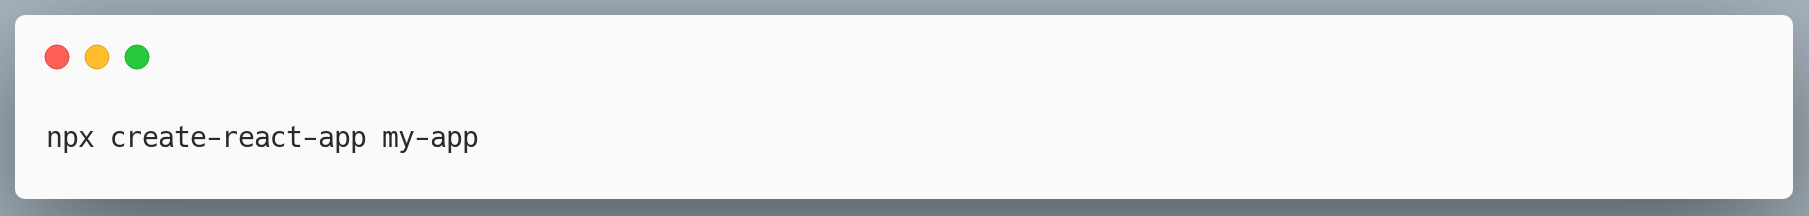
\includegraphics[width=1\textwidth]{./Imagenes/9.1.png}
    \caption[Instalar Create React App]{Instalar Create React App}
    \end{figure}
\newline

Crearemos la web llamada ejemplo-1 con el siguiente comando.
\newline
\begin{figure}[H]
    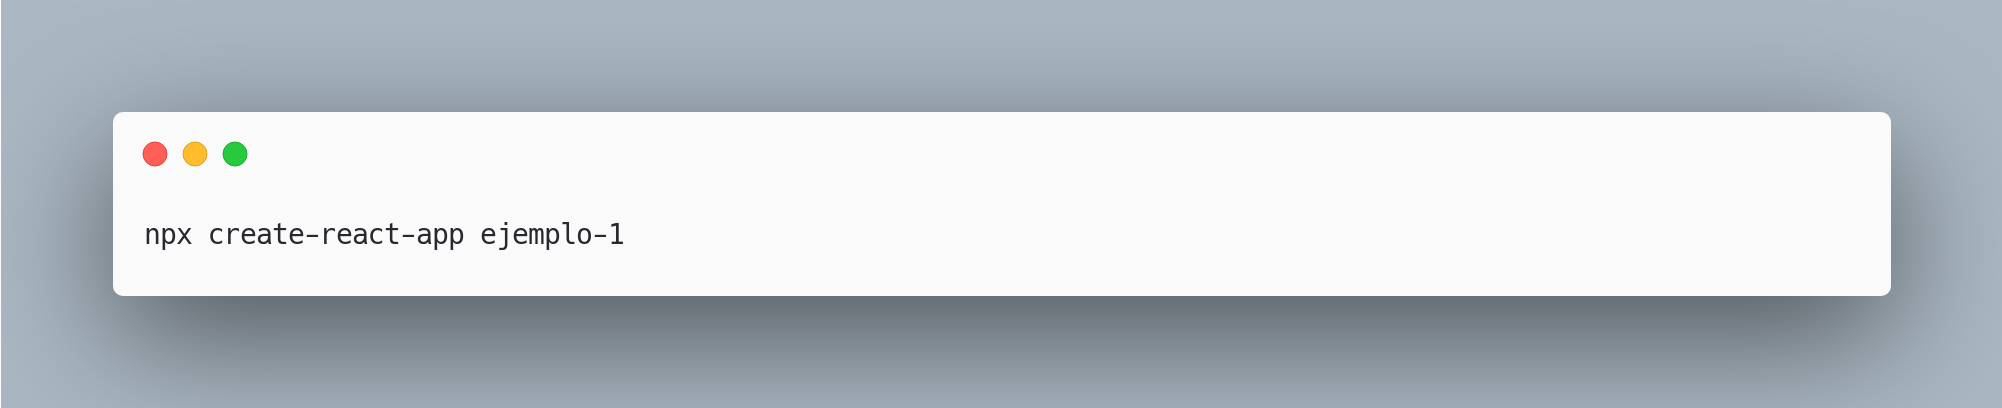
\includegraphics[width=1\textwidth]{./Imagenes/9.2.png}
    \caption[Crear una nueva app]{Crear una nueva app}
    \end{figure}
\newline

El comando nos generará los siguientes directorios.
\newline
\begin{figure}[H]
    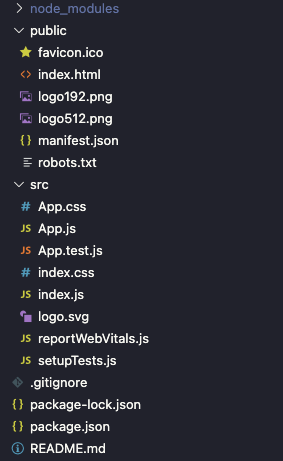
\includegraphics[width=0.5\textwidth]{./Imagenes/9.3}
   \centering 
    \caption[Directorios al crear una nueva app]{Directorios al crear una nueva app}
    \end{figure}
\newline

Para poder probar nuestra librería debemos a indicar a la app ejemplo-1 que use la dependencia desde el modo local, esto con el siguiente comando.\newline
\begin{figure}[H]
    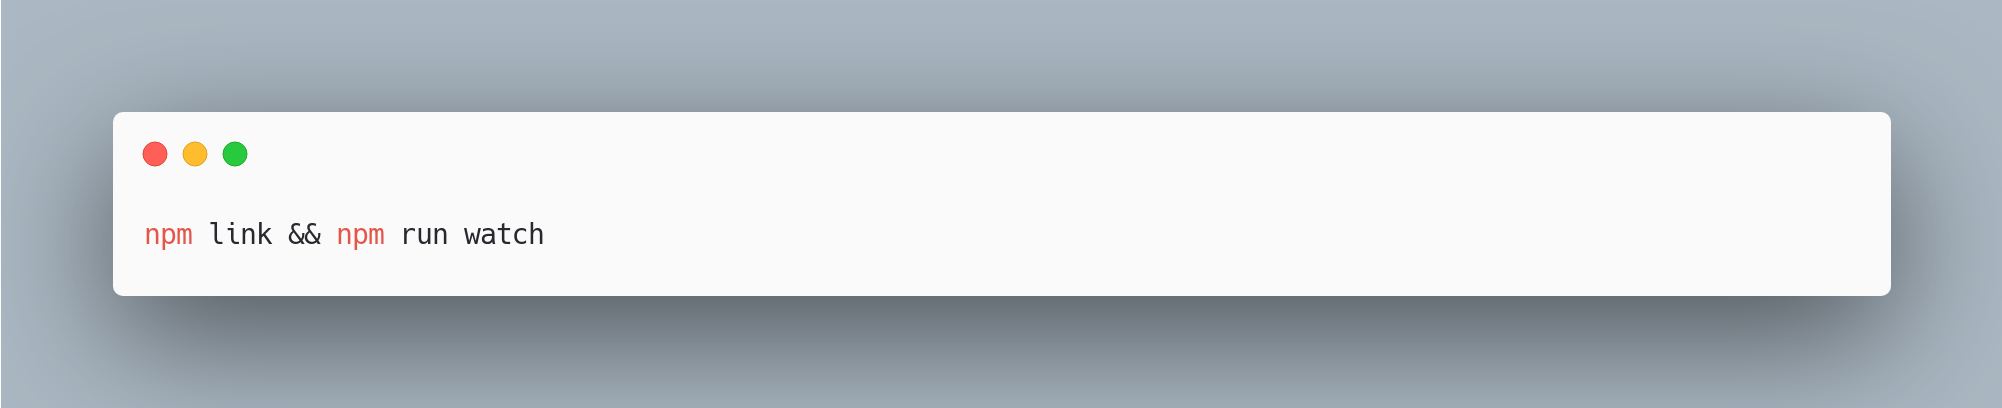
\includegraphics[width=1\textwidth]{./Imagenes/9.4.png}
   \centering 
    \caption[Hacer el puente de manera local]{Hacer el puente de manera local}
    \end{figure}
\newline
Con esto ya es posible usar la librería en cualquier proyecto local.

Dentro del proyecto ejemplo-1 debemos ejecutar el siguiente comando para incluirlo.
\begin{figure}[H]
    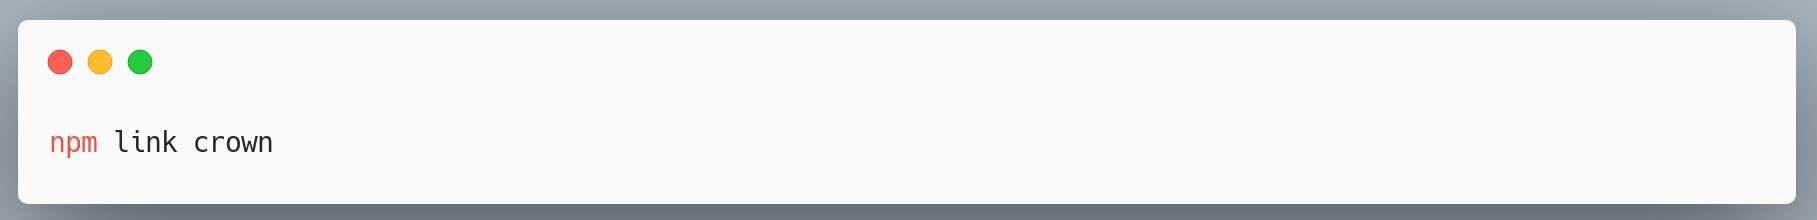
\includegraphics[width=1\textwidth]{./Imagenes/9.5.png}
   \centering 
    \caption[Usar la librería en la aplicación]{Usar la librería en la aplicación}
    \end{figure}
\newline

Ahora basta incluirlo como se agrega cualquier dependencia de node, basta con agregar cualquiera de los elementos aquí desarrollados.
El siguiente código incluye en la primera línea, la importación del componente Label, si se quisieran agregar más, debe enlistarse espaciado por una coma. Y en la parte del return se agrega el componente. Este elemento desplegará un texto por defecto en el navegador.
\begin{figure}[H]
    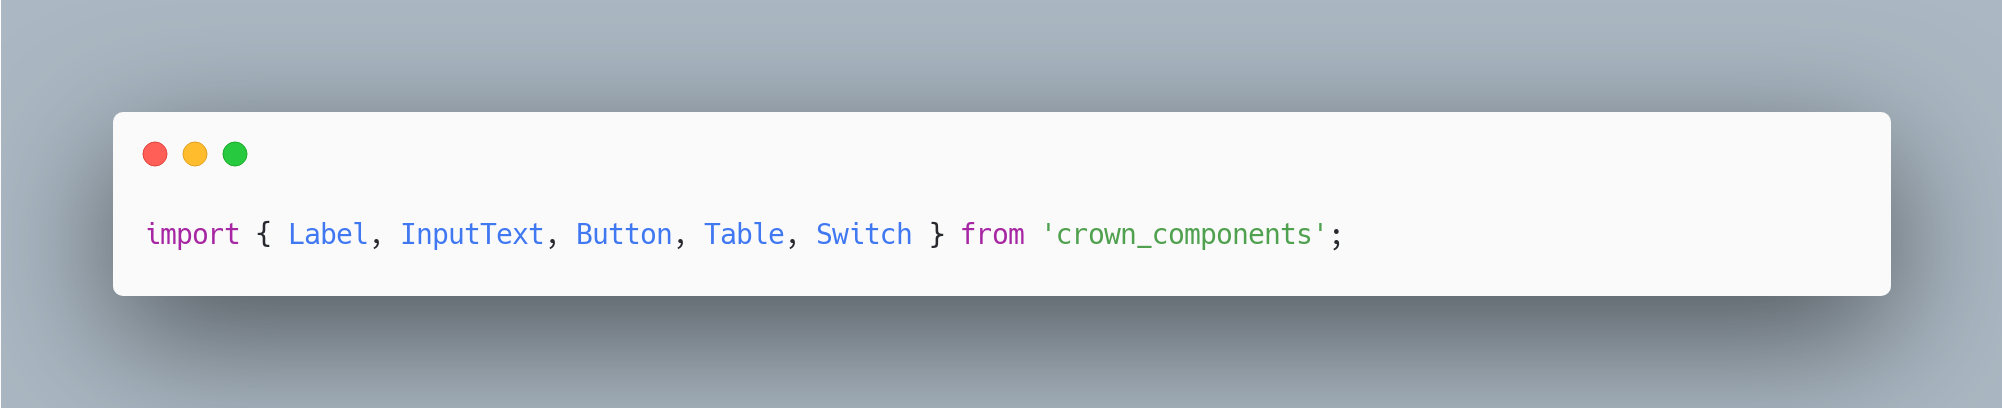
\includegraphics[width=1\textwidth]{./Imagenes/9.6.png}
   \centering 
    \caption[Implementación la librería]{Implementación la librería}
    \end{figure}
\newline